%
% ueberbestimmt.tex
%
% (c) 2018 Prof Dr Andreas Müller, Hochschule Rapperswil
%
\section{Überbestimmte Gleichungssysteme -- ``Least Squares''%
\label{section:ueberbestimmt}}
\index{Gleichungssystem!überbestimmtes}
Bei einem überbestimmten Gleichungssystem, also einem Gleichungssystem
mit mehr Gleichungen als Unbekannten, kann man im Allgemeinen nicht davon
ausgehen, dass es überhaupt eine Lösung gibt.
Ein solches Gleichungssystem hat die Form
\[
A v= b,
\]
wobei $A$ eine Matrix ist, die mehr Zeilen als Spalten hat.

Betrachten wir als Beispiel das Gleichungssystem
\[
\begin{pmatrix}
 6&14\\
12&28\\
 9&21
\end{pmatrix}
\begin{pmatrix}v_1\\v_2\end{pmatrix}
=
\begin{pmatrix}2\\4\\4\end{pmatrix}.
\]
Die Bildmenge der Abbildungsmatrix $A$ beschreibt eine Ebene durch
den Nullpunkt mit den Parametern $v_1$ und $v_2$.
Das Gleichungssystem sucht also nach den Parametern $v_1$ und $v_2$
des Punktes auf der Ebene mit den Koordinaten $(2,4,4)$.
Solche Parameterwerte müssen aber gar nicht existieren, es ist
ja nicht klar, dass der Punkt überhaupt auf der Ebene liegt.

Das Beispiel zeigt aber noch eine weitere Schwierigkeit.
Die beiden Spaltenvektoren von $A$ sind nämlich linear abhängig,
die zweite Spalte ist das $\frac{7}{3}$-fache der ersten Spalte.
Der Rang der Matrix ist daher $1$, die Bildmenge ist sogar nur
eine Gerade.
Man erkennt zum Beispiel, dass der Punkt $(2,4,3)$ auf der Geraden
liegt.
Der gegebene Punkt $(2,4,4)$ kann aber nicht auf der Geraden liegen.
Das Gleichungssystem ist nicht lösbar.

\rhead{Überbestimmte Gleichungssysteme}
%
% Lösungen im Sinne des kleinsten Abstandes
%
\subsection{Lösung im Sinne des kleinsten Abstandes}
Das beste, was man erwarten kann, ist ein Vektor $v_0$ so, dass
der Abstand des Punktes $ b$ von der Ebene (Gerade) bestehend
aus allen $Av$ für $v=v_0$ am kleinsten wird.
Dies geschieht natürlich genau dann, wenn der Differenzvektor $b-Av_0$ auf
allen Vektoren von $Av$ senkrecht steht.

Die Menge der Vektoren der Form $Av$ wird von den Spalten von $A$
aufgespannt.
Es genügt also zu testen, ob $b-Av_0$ auf diesen
Vektoren senkrecht steht.
Dazu müssen die Skalarprodukte von
Spalten von $A$ mit dem Vektor $b-Av_0$ verschwinden, oder
\[
A^t(b-Av_0)=0
\quad
\Rightarrow
\quad
A^tAv_0=A^tb
\]
wir haben also ein Gleichungssystem gefunden mit Matrix $A^tA$ und
rechter Seite $A^tb$, welches als Lösung den gesuchten Vektor
$v_0$ hat.
$A^t$ hat so viele Zeilen wie $v$ Komponenten hat, also
handelt es sich um ein Gleichungssystem mit gleich vielen Gleichungen
wie Unbekannten.
Es wird im Allgemeinen eine eindeutig bestimmte Lösung haben.

\begin{satz} Sei $A$ eine $n\times m$ Matrix und $b$ ein $n$-dimensionaler
Vektor.
Eine Lösung im Sinne minimaler quadrierter Abstände
$
(Av-b)\cdot(Av-b)
$
ist Lösung des Gleichungssystems
\[
A^tAv=A^tb
\]
mit $m$ Gleichungen und $m$ Unbekannten.
\end{satz}

\begin{beispiel}
Man finden den Fusspunkt des Lotes vom Punkt $P=(9,10,7)$ auf die Ebene
durch $O$, $A=(8,10,10)$ und $B=(9,13,12)$.

Der Fusspunkt des Lotes ist der Punkt der Ebene, der den geringsten
Abstand zu $P$ hat.
Die Ebenengleichung ist
\[
A\begin{pmatrix}s\\t\end{pmatrix}=
\begin{pmatrix}
 8& 9\\
10&13\\
10&12
\end{pmatrix}
\begin{pmatrix}s\\t\end{pmatrix}.
\]
Gesucht wird die ``beste Lösung'' von
\[
A\begin{pmatrix}s\\t\end{pmatrix}=\begin{pmatrix}9\\10\\7\end{pmatrix}=b
\]
Dazu muss zunächst die Matrix $A^tA$ und der Vektor $A^tb$
berechnet werden.
\[
A^tA=\begin{pmatrix}
264&322\\
322&394
\end{pmatrix}
,\qquad
A^tb=\begin{pmatrix}
242\\295
\end{pmatrix}.
\]
Daraus findet man die Lösung für $s$ und $t$ numerisch zu
\[
\begin{pmatrix}s\\t \end{pmatrix}
=
\begin{pmatrix}
   1.07831\\
  -0.13253
\end{pmatrix}
\]
und durch Einsetzen in die Ebenengleichung den Ortsvektor des Fusspunktes
\[
\vec f = \begin{pmatrix}
   7.4337\\
   9.0602\\
   9.1928
\end{pmatrix}.
\]
Man kann dieses Resultat dadurch kontrollieren, dass man nachrechnet, ob
$\vec p-\vec f$ senkrecht auf beiden Richtungsvektoren der Ebene
steht:
\[
(\vec p-\vec f)^tA=\begin{pmatrix}
  -1.7451\cdot10^{-11}&  -2.1316\cdot 10^{-11}
\end{pmatrix},
\]
im Rahmen der Rechengenauigkeit steht die Differenz also tatsächlich auf
den Richtungsvektoren senkrecht.
\end{beispiel}

%
% Alles in einem Schritt
%
\subsection{``Alles in einem Schritt''}
In Kapitel~\ref{chapter:affin} wurde gezeigt, wie man Probleme der
affinen Geometrie mit nur einer Durchführung des Gauss-Algorithmus
lösen konnte.
Bei der soeben vorgestellten Lösung des Fusspunkt-Problems
musste man aber wieder in mehrere Schritten vorgehen.
Zuerst wurden $s$ und $t$ bestimmt,
erst in einem zweiten Schritt konnte der Fusspunkt des Lotes
berechnet werden.

Natürlich ist das auch für dieses Problem möglich, man behandelt
$x$, $y$ und $z$ einfach als zusätzliche Variablen, die als Koordinaten
von $Av$ berechnet werden.
Das Gauss-Tableau dazu ist
\[
\begin{tabular}{|>{$}c<{$}>{$}c<{$}>{$}c<{$}>{$}c<{$}|>{$}c<{$}|}
\hline
x&y&z&s\quad t&\\
\hline
1&0&0&        &0\\
0&1&0&-A   &0\\
0&0&1&        &0\\
\hline
 & & &A^tA    &A^tb\\
\hline
\end{tabular}
\]
\begin{beispiel}
Für das Zahlenbeispiel lautet dieses Gauss-Tableau:
\[
\begin{tabular}{|>{$}c<{$}>{$}c<{$}>{$}c<{$}>{$}c<{$}>{$}c<{$}|>{$}c<{$}|}
\hline
x&y&z&s  &  t&\\
\hline
1&0&0& -8& -9&0\\
0&1&0&-10&-13&0\\
0&0&1&-10&-12&0\\
\hline
0&0&0&264&322&242\\
0&0&0&322&394&295\\
\hline
\end{tabular}
\rightarrow
\begin{tabular}{|>{$}c<{$}>{$}c<{$}>{$}c<{$}>{$}c<{$}>{$}c<{$}|>{$}r<{$}|}
\hline
x&y&z&s  &  t&\\
\hline
1&0&0&0&0&7.4337\\
0&1&0&0&0&9.0602\\
0&0&1&0&0&9.1928\\
\hline
0&0&0&1&0&1.0783\\
0&0&0&0&1&-0.1325\\
\hline
\end{tabular}
\]
Man erhält also genau die bereits früher gefundenen Lösungen.
\end{beispiel}

%
% Der allgemein Fall
%
\subsection{Der allgemeine Fall}
Überbestimmte Gleichungssysteme sind Gleichungssysteme der Form
$Ax=b$ mit einer $m\times n$-Matrix mit $m>n$, also mehr Gleichungen
als Unbekannten.
Im Allgemeinen sind sie nicht lösbar, weil $b$ nicht
im Bild von $A$ enthalten ist: $b\not\in \operatorname{im}A$.

Statt einer exakten Lösung könnte man daher eine approximative
Lösung suchen, welche die Gleichung möglichst gut erfüllt.
Der Vektor $Ax-b$ sollte also möglichst kurz sein.
Geometrisch
geht es also darum, das Lot vom Punkt $b$ auf den von den Spaltenvektoren
von $A$ aufgespannten Unterraum zu fällen.
Wir suchen also
einen Vektor, der auf allen Spaltenvektoren von $A$ senkrecht steht.
Das Skalarprodukt von Spaltenvektoren von $A$ mit $Ax-b$ ist aber
$A^t(Ax-b)$, wir müssen also das Gleichungssystem
\[A^t(Ax-b)=0\]
lösen.
Nach Ausmultiplizieren bekommen wir
\begin{equation}
A^tAx-A^tb=0\quad\Rightarrow\quad A^tAx=A^tb\quad\Rightarrow\quad
x=(A^tA)^{-1}A^tb.
\label{uberbestimmt}
\end{equation}
Man beachte, dass $A$ nicht quadratisch ist, und dass man daher
nicht mit $(A^tA)^{-1}A^t=A^{-1}(A^t)^{-1}A^t=A^{-1}$ vereinfachen
kann.

\begin{beispiel}
Sei 
\[
A=\begin{pmatrix}1\\1\\1\\\end{pmatrix},\quad b=\begin{pmatrix}1\\2\\3\end{pmatrix}.
\]
Offenbar ist $b\not\in\operatorname{im}A$.
Nach der Formel (\ref{uberbestimmt}) muss man zunächst $A^tA$ ausrechnen:
\[
A^tA=\begin{pmatrix}1&1&1\end{pmatrix}\begin{pmatrix}1\\1\\1\end{pmatrix}=3.
\]
Damit kann man jetzt nach (\ref{uberbestimmt}) die bestmögliche
approximative Lösung finden:
\[
x=\frac13\cdot\begin{pmatrix}1&1&1\end{pmatrix}
\begin{pmatrix}1\\2\\3\end{pmatrix}=2.
\]
Der von $b$ am wenigsten weit entfernte Punkt der Geraden mit
Richtung $A$ ist also der Punkt $(2,2,2)$.
\end{beispiel}

%
% Anwendungen der Methode der kleinsten Quadrate
%
\subsection{Anwendungen der Methode der kleinsten Quadrate}
Die Bedeutung der Methode der kleinsten Qudarate besteht darin, dass 
man in der Praxis sehr oft die Situation hat, dass man deutlich mehr
Daten hat als nötig, um die Parameter eines Problems zu bestimmen.
Zum Beispiel genügt es, drei Punkte eines Kreises zu kennen, um
Mittelpunkt und Radius exakt bestimmen zu können.
Oder zwei Punkte bestimmen eine Gerade eindeutig.
In der Praxis misst man meistens mehr Punkte.
Allerdings sind die Messungen mit Messfehlern behaftet.
Die Methode der kleinsten Quadrate erlaubt dann, die bestmöglichen
Werte für die Parameter zu finden.
Dies soll an zwei Beispielen illustriert werden.

\subsubsection{Gerade durch Punkte}
\begin{figure}
\centering
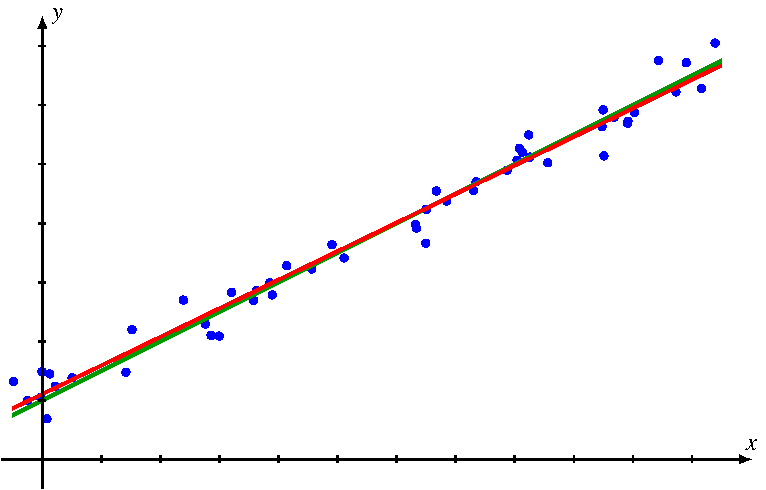
\includegraphics{4/images/linreg.pdf}
\caption{Bestimmung einer Geraden, die eine Menge von Punkten am besten
approximiert.
Die blauen Punkte sind entstanden, indem Punkte der grünen Gerade
mit einer zufälligen Abweichungen gestört wurden.
Die rot eingezeichnete Regeressionsgerade approximiert die ursprüngliche
Gerade mit grosser Genauigkeit.
\label{skript:linreg-abb}}
\end{figure}
Gegeben sind Punkte $(x_i,y_i)$ mit $1\le i\le n$, die ungefähr auf
einer Geraden $y={\color{red}a}x+{\color{red}b}$ liegen.
Gesucht sind die Werte von $\color{red}a$ und $\color{red}b$
(Abbildung~\ref{skript:linreg-abb}).
Zur Verdeutlichung heben wir im
Folgenden die Unbekannten rot hervor.
Wären die Punkte exakt auf der Geraden, müsste jeder die Geradengleichung
erfüllen, wir erhielten also die Gleichungen
\begin{equation}
\begin{linsys}{2}
{\color{red}a}x_1&+     &{\color{red}b}&=&y_1\\
{\color{red}a}x_2&+     &{\color{red}b}&=&y_2\\
                 &\vdots&              & &\vdots\hspace*{1mm}\\
{\color{red}a}x_n&+     &{\color{red}b}&=&y_n
\end{linsys}
\label{leastsquares:gerade}
\end{equation}
Dies ist ein Gleichungssystem für die Unbekannten ${\color{red}a}$ und
${\color{red}b}$ mit $n$
Gleichungen, im Allgemeinen ist es also überbestimmt.

Die Gleichung \eqref{leastsquares:gerade} kann mit dem Standardverfahren
gelöst werden.
Dazu schreiben wir zunächst die Matrix $A$ und den Vektor $b$ auf:
\[
A
=
\begin{pmatrix}
x_1   &1     \\
x_2   &1     \\
\vdots&\vdots\\
x_n   &1
\end{pmatrix}
,\qquad
x=
\begin{pmatrix}
\color{red}a\\
\color{red}b
\end{pmatrix},
\qquad
b
=
\begin{pmatrix}
y_1\\
y_2\\
\vdots\\
y_n
\end{pmatrix}
\]
Für die Lösung müssen wir $A^tA$ und $A^tb$ berechnen:
\begin{align*}
A^tA
&=
\begin{pmatrix}
x_1&x_2&\dots&x_n\\
 1 & 1 &\dots& 1
\end{pmatrix}
\begin{pmatrix}
x_1   &1     \\
x_2   &1     \\
\vdots&\vdots\\
x_n   &1
\end{pmatrix}
=
\begin{pmatrix}
\displaystyle\sum_{i=1}^n x_i^2 & \displaystyle\sum_{i=1}^n x_i \\
\displaystyle\sum_{i=1}^n x_i   &       n
\end{pmatrix}
\\
A^tb
&=
\begin{pmatrix}
x_1&x_2&\dots&x_n\\
 1 & 1 &\dots& 1
\end{pmatrix}
\begin{pmatrix}
y_1\\
y_2\\
\vdots\\
y_n
\end{pmatrix}
=
\begin{pmatrix}
\displaystyle \sum_{i=1}^n x_iy_i\\
\displaystyle \sum_{i=1}^n y_i
\end{pmatrix}.
\end{align*}
Die Determinante von $A^tA$ ist
\[
\det(A^tA)
=
n\sum_{i=1}^n x_i^2 -\biggl(\sum_{i=1}^n x_i\biggr)^2
.
\]
Dieses Gleichungssystem kann man jetzt mit der Cramerschen Regel für die
Unbekannte ${\color{red}a}$ lösen:
\begin{align*}
{\color{red}a}
&=
\frac{\displaystyle
n\sum_{i=1}^n x_iy_i-\sum_{i=1}^nx_i\sum_{i=1}^ny_i
}{\displaystyle
n\sum_{i=1}^n x_i^2 -\biggl(\sum_{i=1}^n x_i\biggr)^2
}
=
\frac{\displaystyle
\frac1n\sum_{i=1}^n x_iy_i-\frac1n\sum_{i=1}^nx_i\cdot \frac1n\sum_{i=1}^ny_i
}{\displaystyle
\frac1n\sum_{i=1}^n x_i^2 -\biggl(\frac1n\sum_{i=1}^n x_i\biggr)^2
}.
\end{align*}
Den Achsenabschnitt $\color{red}b$ könnte man natürlich auch so finden,
es geht aber auch direkter.
Bildet man die Summe der Gleichungen 
\ref{leastsquares:gerade}, erhält man
\[
{\color{red}a}
\sum_{i=1}^n x_i
+
n{\color{red}b}
=
\sum_{i=1}^n y_i.
\]
Auflösen nach $\color{red}b$ ergibt
\begin{align*}
{\color{red}b}
&=
\frac1n\sum_{i=1}^n y_i
-{\color{red}a}
\cdot
\frac1n\sum_{i=1}^n x_i.
\end{align*}
Die so gefundene Gerade  mit der Gleichung
$y={\color{red}a}x+{\color{red}b}$
heisst auch {\em Regressionsgerade}.
\index{Regressionsgerade}

\subsubsection{Kreis durch Punkte}
\begin{figure}
\centering
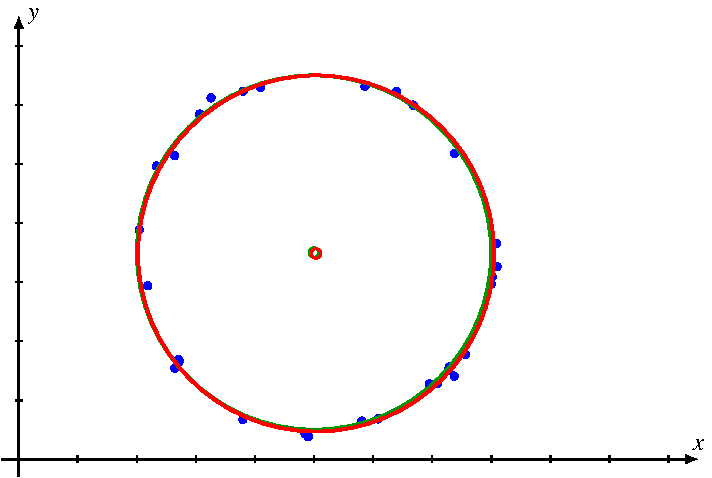
\includegraphics{4/images/kreis.pdf}
\caption{Bestimmung eines Kreises, der eine Menge von Punkten am besten
approximiert.
Die blauen Punkte sind entstanden, indem Punkte des grünen Kreises
mit einer zufälligen Abweichungen gestört wurden.
Der rot eingezeichnete Kreis approximiert den ursprünglichen
Kreis mit grosser Genauigkeit.
\label{skript:linreg-abb}}
\end{figure}
Gegeben sind die Punkte $(x_i,y_i)$ mit $1\le i\le n$, die ungefähr
auf einem Kreis liegen.
Gesucht sind Mittelpunkt $M=(m_x,m_y)$ und Radius $r$ dieses Kreises.
Wieder heben wir zur Verdeutlichung im Folgenden die Unbekannten farbig
hervor.
Zunächst müssen wir Gleichungen für die gesuchten Variablen aufstellen.
Die Gleichung eines Kreises ist
\[
(x_i - {\color{red}m_x})^2 + (y_i - {\color{red}m_y})^2 = {\color{red}r}^2.
\]
Diese Gleichungen sind allerdings nicht linear.
Das Standardverfahren ist also nicht anwendbar.
Wir multiplizieren daher aus, und erhalten
\[
x_i^2 - 2x_i {\color{red}m_x} + {\color{red}m_x}^2
+
y_i^2 - 2y_i {\color{red}m_y} + {\color{red}m_y}^2
=
{\color{red}r}^2.
\]
Indem wir die Quadrate der Variablen zu einer neuen Variable 
\[
{\color{red}c}
=
{\color{red}r}^2
-
{\color{red}m_x}^2
-
{\color{red}m_y}^2
\]
zusammenfassen, können wir die Gleichungen in lineare Form bringen:
\begin{equation}
2x_i{\color{red}m_x}
+
2y_i{\color{red}m_y}
+
{\color{red}c}
=
x_i^2+y_i^2,\qquad 1\le i\le n.
\end{equation}
In dieser Form lässt sich das Standardverfahren anwenden, die Matrix
$A$ und die Vektoren $x$ und $b$ sind
\begin{align*}
A
&=
\begin{pmatrix}
2x_1  & 2y_1 & 1    \\
2x_2  & 2y_2 & 1    \\
\vdots&\vdots&\vdots\\
2x_n  & 2y_n & 1    \\
\end{pmatrix},
&
x&=\begin{pmatrix}
{\color{red}m_x}\\
{\color{red}m_y}\\
{\color{red}c}
\end{pmatrix}
&&\text{und}&
b
&=
\begin{pmatrix}
x_1^2+y_1^2\\
x_2^2+y_2^2\\
\vdots\\
x_n^2+y_n^2
\end{pmatrix}.
\end{align*}
Aus der Lösung kann dann der Radius als 
\[
{\color{red}r}= 
\sqrt{
{\color{red}c}
+
{\color{red}m_x}^2
+
{\color{red}m_y}^2
}
\]
bestimmt werden.
Abbildung~\ref{skript:linreg-abb} zeigt, wie der Kreis mit grosser
Genauigkeit auch aus stark fehlerbehafteten Punkten bestimmt werden
kann.

\subsubsection{Drehung und Translation finden}
\begin{figure}
\centering
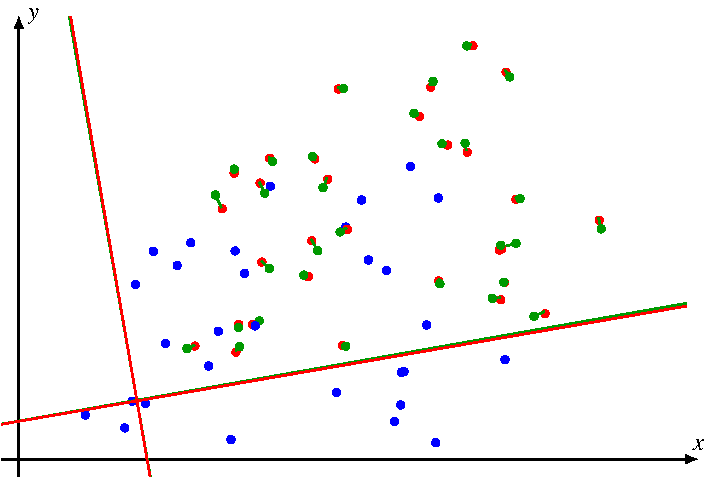
\includegraphics{4/images/bewegung.pdf}
\caption{Bestimmung von Drehwinkel und Translation einer Bewegung.
Die ursprüngliche Bewegung bewegt das schwarze Koordinatenkreuz auf
die grünen Achsen.
Die blauen Punkte werden mit dieser Bewegung abgebildet aber zusätzlich
noch mit einem zufälligen Fehler überlagert, so entstehen die grünen Punkte.
Die kurzen grünen Linien beginnen beim exakten Bild eines blauen Punktes.
Das im Text beschriebene Verfahren liefert den Drehwinkel und die
Verschiebung, die das Koordinatensystem auf die roten Achsen bewegt.
Damit werden die blauen Punkte auf die roten Punkte abgebildet.
Es zeigt sich, dass die grünen Linien ziemlich genau dort beginnen, wo
die gefundene Bewegung die blauen Punkte hinbewegt, das Verfahren kann
sowohl die Bewegung als auch die Fehler (die grünen Linien)
recht genau ermitteln.
\label{skript:bewegung-leastsquares}}
\end{figure}
Das Regstrierungsproblem in der Bildverarbeitung verlangt, zwei Bilder
der gleichen Szene mit Hilfe einer Drehung und Translation zur Deckung
zu bringen.
In der Astrophotographie kann man zum Beispiel in zwei Bildern die
Positionen der
Sterne $(x_i,y_i)$ und $(x_i',y_i')$ in jedem Bild finden und dann
die Transformation suchen, die die Punkte möglichst genau zur Deckung bringt.
Diese Transformation kann in Matrixform als
\begin{align*}
\begin{pmatrix}
x_i'\\y_i'
\end{pmatrix}
=
\begin{pmatrix}
\cos{\color{red}\alpha}&-\sin{\color{red}\alpha}& \color{red}t_x\\
\sin{\color{red}\alpha}&\phantom{-} \cos{\color{red}\alpha}& \color{red}t_y
\end{pmatrix}
\begin{pmatrix}
x_i\\y_i\\1
\end{pmatrix}
\end{align*}
geschrieben werden.
Der Winkel ${\color{red}\alpha}$ tritt in den Gleichungen nicht
linear auf.
Stattdessen verwenden wir
${\color{red}c}=\cos{\color{red}\alpha}$
und
${\color{red}s}=\sin{\color{red}\alpha}$
als Unbekannte.
Die Gleichungen werden 
\begin{equation}
\begin{linsys}{6}
x_i{\color{red}c} &-& y_i{\color{red}s} &+& {\color{red}t_x} & &                &=&x_i'\\
y_i{\color{red}c} &+& x_i{\color{red}s} & &                  &+&{\color{red}t_y}&=&y_i'\\
\end{linsys}
\end{equation}
Dies ist ein überbestimmtes lineares Gleichungssystem von
$2n$-Gleichungen für die vier Unbekannten
${\color{red}c}$,
${\color{red}s}$,
${\color{red}t_x}$ und
${\color{red}t_y}$.
Die Matrix $A$ und die Vektor $x$ und $b$ sind
\begin{align*}
A&=
\begin{pmatrix}
x_1&-y_1&1&0\\
y_1& x_1&0&1\\
x_2&-y_2&1&0\\
y_2& x_2&0&1\\
\vdots&\vdots&\vdots&\vdots\\
x_n&-y_n&1&0\\
y_n& x_n&0&1\\
\end{pmatrix},
&
x
&=
\begin{pmatrix}
{\color{red}c}\\
{\color{red}s}\\
{\color{red}t_x}\\
{\color{red}t_y}
\end{pmatrix}
&&\text{und}&
b
&=
\begin{pmatrix}
x_1'\\
y_1'\\
x_2'\\
y_2'\\
\vdots\\
x_n'\\
y_n'\\
\end{pmatrix}
\end{align*}
Es ist nicht garantiert, dass die Lösung
\[
\lambda^2
=
{\color{red}c}^2
+
{\color{red}s}^2
=1
\]
erfüllen wird, wie das für $\cos\alpha$ und $\sin\alpha$ der Fall wäre.
Die Bedeutung von $\lambda$ ist die eines zusätzlichen Streckungsfaktors,
dem das Bild für optimale Deckung auch noch unterworfen werden sollte.
Abbildung~\ref{skript:bewegung-leastsquares} zeigt an einem Beispiel, wie
das Verfahren die Bewegung aus wenigen Punkten ermitteln kann.



